\documentclass[12pt]{article}   % list options between brackets
\usepackage{graphicx}

% type user-defined commands here

\begin{document}

\title{CS288 Assignment 1: Language Model}   % type title between braces
\author{Reynold Shi Xin}         % type author(s) between braces
\date{rxin@cs.berkeley.edu}    % type date between braces
\maketitle

%%%%%%%%%%%%%%%%%%%%%%%%%%%%%%%%%%%%%%%%%%%%%%%%%%%%%%%%%%%%%%%%%%%%%%%
%%%%%%%%%%%%%%%%%%%%%%%%%%%%%%%%%%%%%%%%%%%%%%%%%%%%%%%%%%%%%%%%%%%%%%%
\section{Performance Summary}
I have implemented a trigram language model with Kneser-Ney smoothing. The exact model meets the requirements for both exact and noisy. The following performance metrics are reported on an Amazon EC2 large instance, running Ubuntu 10.04LTS with Sun JDK 1.6:
\begin{enumerate}
	\item BLEU score 24.533 with discounting factor 0.90;
	\item Using hash table load factor 0.8, training takes 300s, decoding takes 300s, memory consumption at 905MB;
	\item Using hash table load factor 0.95, training takes 400s, decoding takes 700s, memory 836MB;
	\item Noisy model counts should be 100\% correct because the model is not ``noisy'' at all.
\end{enumerate}

Note that the above runtime is measured when outputs are printed to stdout. If we re-route output to /dev/null, the speed can be improved further.

Unless otherwise stated, the memory usage number in this report includes the phrase table and vocabulary, which themselves occupy about 300MB.

%%%%%%%%%%%%%%%%%%%%%%%%%%%%%%%%%%%%%%%%%%%%%%%%%%%%%%%%%%%%%%%%%%%%%%%
%%%%%%%%%%%%%%%%%%%%%%%%%%%%%%%%%%%%%%%%%%%%%%%%%%%%%%%%%%%%%%%%%%%%%%%
\section{Code Structure}
This section provides a high level overview of the classes. The code is fairly modular and easy to extend. For example, I made attempts to build a noisy model using approximate hash maps, which does not even require changing the language model code at all.

\begin{enumerate}
	\item \texttt{BigramIndexer}: A hash map that maps a 64-bit bigram (two unigram indexes, 64 bits) to a 32-bit bigram index. It is simply a wrapper around \texttt{CrazilyPackedHashMap}.
	\item \texttt{CrazilyPackedHashMap}: A fast, highly memory efficient hash map. (Section \ref{sec:crazyhashmap})
	\item \texttt{CrazilyPackedHashMapApproximate}: The noisy version of CrazilyPackedHashMap. (Section \ref{sec:noisy})
	\item \texttt{HashFunctions}: Provides various hash functions.
	\item \texttt{KneserNeyTrigramLm}: The Kneser-Ney trigram language model that uses CrazilyPackedHashMap by default. If \\ \texttt{CrazilyPackedHashMapApproximate} is provided, this becomes a noisy model.
	\item \texttt{PrimeFinder}: Provides fast functions to find prime numbers for hash table capacities.
	\item \texttt{TrigramCounter}: A hash map for counting trigram frequencies. It is simply a wrapper around \texttt{CrazilyPackedHashMap}.
	\item \texttt{TrigramCounterApproximate}: A wrapper around \\ \texttt{CrazilyPackedHashMapApproximate}.
	\item \texttt{TrigramCounterInterface}: self-evident.
	\item \texttt{Utils}: Provides functions for packing and unpacking integers.
\end{enumerate}



%%%%%%%%%%%%%%%%%%%%%%%%%%%%%%%%%%%%%%%%%%%%%%%%%%%%%%%%%%%%%%%%%%%%%%%
%%%%%%%%%%%%%%%%%%%%%%%%%%%%%%%%%%%%%%%%%%%%%%%%%%%%%%%%%%%%%%%%%%%%%%%
\section{Quality Parameters}
The main quality parameter to tweak is the discount factor in Kneser-Ney. Although 0.70 -- 0.75 are commonly used, the empirical optimal discount value I found is 0.90 despite the difference is almost negligible. This is also consistent with a quick experiment I conducted to determine the empirical discount, which indicates rare trigrams are less likely to re-appear in this corpus.

Table \ref{tbl:discount} summarizes how discount factor affects the BLUE score.

\begin{table}
\label{tbl:discount}
\centering
\begin{tabular}{ c | c  }
	discount factor & BLUE score \\
	\hline
	0.70 & 24.493 \\
	0.75 & 24.502 \\
	0.80 & 24.520 \\
	0.90 & \textbf{24.533} \\
	0.95 & 24.493
\end{tabular}
\caption{Discount factor and the BLUE score}
\end{table}

Another parameter to tweak is the assumed frequency of unseen trigrams and bigrams. I experimented with some different values and concluded the best value for this corpus is $10^{-6}$.


%%%%%%%%%%%%%%%%%%%%%%%%%%%%%%%%%%%%%%%%%%%%%%%%%%%%%%%%%%%%%%%%%%%%%%%
%%%%%%%%%%%%%%%%%%%%%%%%%%%%%%%%%%%%%%%%%%%%%%%%%%%%%%%%%%%%%%%%%%%%%%%
\section{Optimization Techniques}
I have tried and employed a number of optimization techniques to reduce the memory consumption. Initially, using a naïve implementation that simply stores the language model using Java’s HashMap with closed addressing, the language model would take more than 3 GB of memory to store. This number was cut to less than 1GB using these techniques.

\subsection{Open Addressing Hash Map with Linear Probing}
First and foremost, to reduce the overhead of Java objects, I had to avoid using Java's HashMap implementation, which supports only closed addressing and doesn't allow using primitive types as keys or values.

I tested GNU Trove, which is a fast and lightweight implementation of collections (e.g. hash maps) for primitives. I was able to fit the language model in 1.7G of memory using GNU Trove. At the end, however, I wrote my own hash map implementation for better performance and memory.


\subsection{Hashing Algorithm}
\label{sec:hashing}
I tested out a few hashing algorithms for 64 bit integers. The initial hashing algorithm simply mods the integer by a prime number, which is set to the size of the hash map. The performance was terrible due to a high number of collisions, taking over 60 mins to decode. The CERN (European Organization for Nuclear Research) algorithm produces the best performance :
\begin{verbatim}
((int) (value ^ (value >>> 32))) * 31;
\end{verbatim}

\subsection{Context Encoding for Bigrams}
All words are mapped to a 32-bit integer using the \texttt{StringIndexer} class provided by the instructor. In reality, the corpus only contain half 495,172 unigrams, i.e. 19 bits to store represent unigram.

Because the bigram vector is very sparse (only 8,374,230 bigrams), I exploited context encoding to save space for storing bigrams. A hash map (\texttt{BigramIndexer}) is created to map a bigram (two 32-bit unigrams) to a 23-bit integer.

Using context encoding, I reduced the memory usage to 1.2GB.


\subsection{“Crazily Packed” Hash Map}
\label{sec:crazyhashmap}

\begin{table}
\label{tbl:datasize}
\centering
\begin{tabular}{ c | c | c  }
	data type & value range & bits required \\
	\hline
	unigram index & 495,172 & 19 bits \\
	bigram index & 8,374,230 & 23 bits \\
	trigram frequency & 468,261 & 19 bits
\end{tabular}
\caption{The number of bits required to store data in the language model}
\end{table}

The largest memory reduction comes from the observation that the value of most counters or indexers in the language model do not require full 32-bit integers to store (Table \ref{tbl:datasize}).

For example, for the \texttt{TrigramCounter}, which maps a trigram to the number of times the trigram appears. The key is composed of a bigram index (for the first two words) and an unigram index (for the third word). The value is a 32-bit counter. An entry in a regular hash map would take 96 bits of space.

Based on Table \ref{tbl:datasize}, a single 61-bit integer (\texttt{long}) is enough to store information for both the key and value of an element in the \texttt{TrigramCounter}. In the \texttt{TrigramCounter} hash map, rather than using two separate arrays to store the key (two 32 bit integers) and the value (one 32 bit integer) respectively, we pack both the key array and the value array into a single 64 bit integer array, as shown in Figure \ref{fig:trigramcounter}.

\begin{figure}[h*]
	\centering
	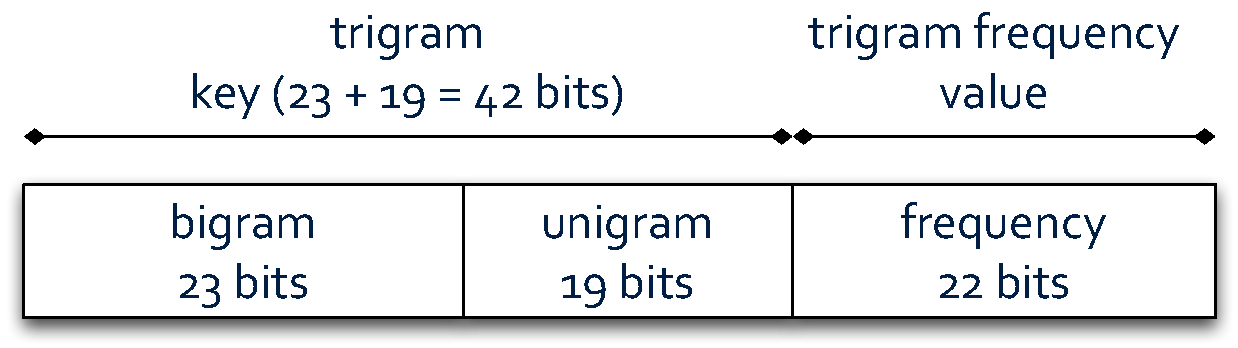
\includegraphics[width=10cm]{trigram_map.pdf}
	\caption{An element in the \texttt{TrigramCounter}}
	\label{fig:trigramcounter}
\end{figure}

Table \ref{tbl:perf} illustrates the decoding time and the memory usage using various hash map load factors. The decoding time is relatively constant when the load factor is below 0.70. Once the load factor goes beyond 0.75, the performance degrades linearly because of collision. When the load factor is above 0.90, collision becomes severe and performance degradation is very evident.

A somewhat surprising result is despite the bit manipulations, the runtime performance actually improved by using this hash map. Although it’s hard to verify, I suspect the speed improvement is due to higher cache hits and lower page faults thanks to the smaller data structure size.

\begin{table}
\label{tbl:perf}
\centering
\begin{tabular}{ c | c | c  }
	load factor & decoding time & memory usage \\
	\hline
	0.70 & 300s & 997M \\
	0.75 & 315s & 950M \\
	0.80 & 311s & 905M \\
	0.85 & 331s & 881M \\
	0.90 & 354s & 861M \\
	0.95 & 700s & 836M \\
\end{tabular}
\caption{Hash Map Load Factor vs Performance and Memory Usage. The decoding time includes writing output to \texttt{stdout}. The memory usage includes phrase tables and vocabulary, which themselves occupy about 300MB.}
\end{table}


\subsection{Pre-allocated Data Structures}
To improve the training speed, the language model pre-allocates a large amount of memory to all counters to avoid the re-hashing and dynamic growing of data structures. To pass the sanity test, which only allows 50 MB of max heap space, the language model checks what the max heap size is, and allocates a smaller amount of memory if the max heap size is less than 500 MB.

This optimization technique does not affect the memory consumption and the decoding speed. It does however reduce the training time and allows me to iterate through different algorithms and optimization techniques much faster.

%%%%%%%%%%%%%%%%%%%%%%%%%%%%%%%%%%%%%%%%%%%%%%%%%%%%%%%%%%%%%%%%%%%%%%%
%%%%%%%%%%%%%%%%%%%%%%%%%%%%%%%%%%%%%%%%%%%%%%%%%%%%%%%%%%%%%%%%%%%%%%%
\section{Attempts for Noisy Model}
\label{sec:noisy}
Although my exact model also meets the requirements for the noisy model, I spent some efforts in designing noisy models that further reduce memory. Because my program is well structured, I felt the best way to attempt a noisy model was to design an approximate hash map. This would require no change to the language model code, only touching the part that initialize the hash maps.

To compress the hash map, I use only a 32-bit integer array, which consists of a hash code of the key (9 bits), and the value. Because the key hash code contains only 9 bits of information, there is a potential collision here. The approximation simply ignores the collision. The hash code of the key is:
\begin{verbatim}
((int) (key ^ (key >>> 32))) % 509;
\end{verbatim}

Note that the above hash function is different from the hash function used to compute the location of the element. To compute the location of the element, the hash function in Section \ref{sec:hashing} is used.

\begin{figure}[h*]
	\centering
	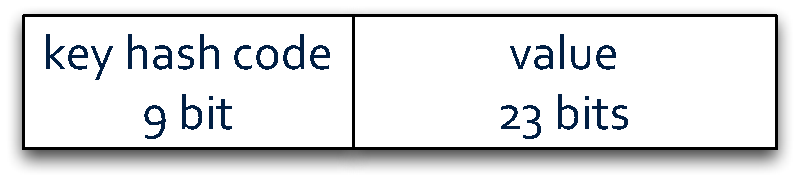
\includegraphics[width=6cm]{noisy_map.pdf}
	\caption{An element in the noisy, approximate hash map}
	\label{fig:noisy_map}
\end{figure}

I was able to reduce the memory usage to 700MB using the approximate hash map. However, the BLEU score also dropped to slightly below 22 due to too much collision.

If I had spent more time in finding a better hash function, I could probably reduce the degree of collision. However, because the exact model already meets the requirement, I did not spend extra time and decided to use the exact model for the ``NOISY'' implementation.






\end{document}
